\begin{figure*}[t]
\centering
\resizebox{\linewidth}{!}{%
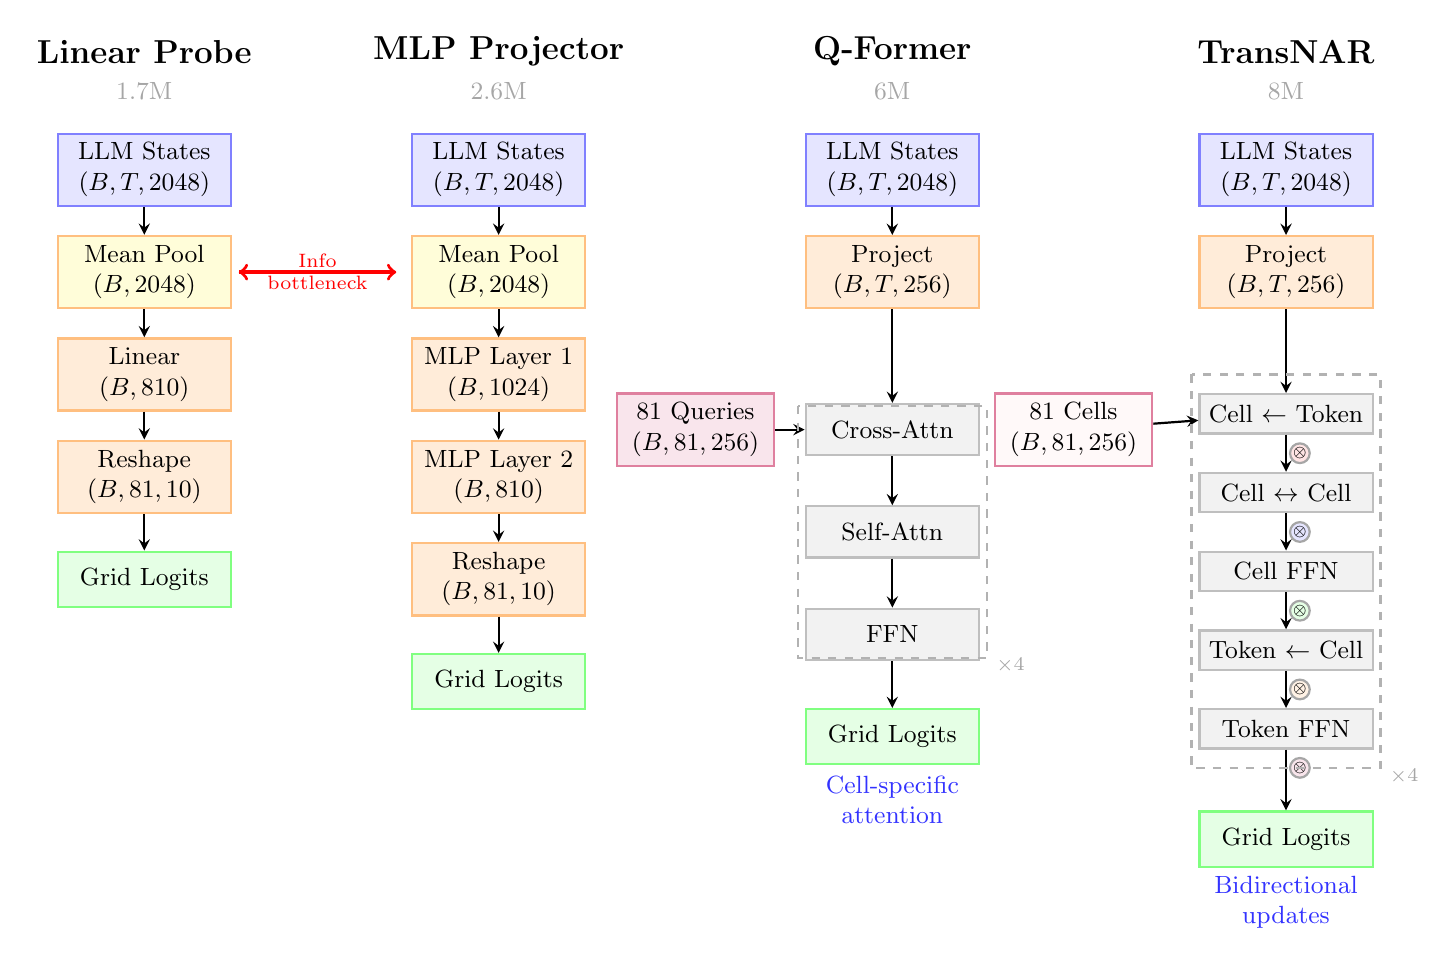
\begin{tikzpicture}[
    box/.style={rectangle, draw, thick, minimum width=2.2cm, minimum height=0.7cm, align=center, font=\small},
    input/.style={box, fill=blue!10, draw=blue!50},
    output/.style={box, fill=green!10, draw=green!50},
    pool/.style={box, fill=yellow!15, draw=orange!50},
    linear/.style={box, fill=orange!15, draw=orange!50},
    query/.style={box, fill=purple!10, draw=purple!50, minimum width=2.0cm},
    attn/.style={box, fill=gray!10, draw=gray!50, minimum height=0.65cm},
    arrow/.style={->, >=stealth, thick},
    title/.style={font=\large\bfseries},
    params/.style={font=\small, color=gray!70}
]

% Architecture 1: Linear Probe
\node[title] at (0, 0) {Linear Probe};
\node[params] at (0, -0.5) {1.7M};
\node[input] (in1) at (0, -1.5) {LLM States\\$(B,T,2048)$};
\node[pool] (pool1) at (0, -2.8) {Mean Pool\\$(B,2048)$};
\node[linear] (lin1) at (0, -4.1) {Linear\\$(B,810)$};
\node[linear] (reshape1) at (0, -5.4) {Reshape\\$(B,81,10)$};
\node[output] (out1) at (0, -6.7) {Grid Logits};
\draw[arrow] (in1) -- (pool1);
\draw[arrow] (pool1) -- (lin1);
\draw[arrow] (lin1) -- (reshape1);
\draw[arrow] (reshape1) -- (out1);
\node[font=\scriptsize, color=red, align=center] at (2.2, -2.8) {Info\\bottleneck};
\draw[->, red, very thick] (1.8, -2.8) -- (1.2, -2.8);
\draw[<-, red, very thick] (3.2, -2.8) -- (1.2, -2.8);

% Architecture 2: MLP Projector
\node[title] at (4.5, 0) {MLP Projector};
\node[params] at (4.5, -0.5) {2.6M};
\node[input] (in2) at (4.5, -1.5) {LLM States\\$(B,T,2048)$};
\node[pool] (pool2) at (4.5, -2.8) {Mean Pool\\$(B,2048)$};
\node[linear] (mlp2a) at (4.5, -4.1) {MLP Layer 1\\$(B,1024)$};
\node[linear] (mlp2b) at (4.5, -5.4) {MLP Layer 2\\$(B,810)$};
\node[linear] (reshape2) at (4.5, -6.7) {Reshape\\$(B,81,10)$};
\node[output] (out2) at (4.5, -8.0) {Grid Logits};
\draw[arrow] (in2) -- (pool2);
\draw[arrow] (pool2) -- (mlp2a);
\draw[arrow] (mlp2a) -- (mlp2b);
\draw[arrow] (mlp2b) -- (reshape2);
\draw[arrow] (reshape2) -- (out2);

% Architecture 3: Q-Former
\node[title] at (9.5, 0) {Q-Former};
\node[params] at (9.5, -0.5) {6M};
\node[input] (in3) at (9.5, -1.5) {LLM States\\$(B,T,2048)$};
\node[linear] (proj3) at (9.5, -2.8) {Project\\$(B,T,256)$};
\node[query] (q3) at (7.0, -4.8) {81 Queries\\$(B,81,256)$};
\node[attn] (cross3) at (9.5, -4.8) {Cross-Attn};
\node[attn] (self3) at (9.5, -6.1) {Self-Attn};
\node[attn] (ffn3) at (9.5, -7.4) {FFN};
\node[output] (out3) at (9.5, -8.7) {Grid Logits};
\draw[arrow] (in3) -- (proj3);
\draw[arrow] (proj3) -- (cross3);
\draw[arrow] (q3) -- (cross3);
\draw[arrow] (cross3) -- (self3);
\draw[arrow] (self3) -- (ffn3);
\draw[arrow] (ffn3) -- (out3);
\draw[dashed, gray!60, thick] (8.3, -4.5) rectangle (10.7, -7.7);
\node[font=\scriptsize, gray!70] at (11.0, -7.8) {$\times$4};
\node[font=\small, color=blue!80, align=center] at (9.5, -9.5) {Cell-specific\\attention};

% Architecture 4: TransNAR
\node[title] at (14.5, 0) {TransNAR};
\node[params] at (14.5, -0.5) {8M};
\node[input] (in4) at (14.5, -1.5) {LLM States\\$(B,T,2048)$};
\node[linear] (proj4) at (14.5, -2.8) {Project\\$(B,T,256)$};
\node[query, fill=pink!10] (cell4) at (11.8, -4.8) {81 Cells\\$(B,81,256)$};
\node[attn, minimum height=0.5cm] (gate4a) at (14.5, -4.6) {Cell $\leftarrow$ Token};
\node[attn, minimum height=0.5cm] (gate4b) at (14.5, -5.6) {Cell $\leftrightarrow$ Cell};
\node[attn, minimum height=0.5cm] (ffn4a) at (14.5, -6.6) {Cell FFN};
\node[attn, minimum height=0.5cm] (gate4c) at (14.5, -7.6) {Token $\leftarrow$ Cell};
\node[attn, minimum height=0.5cm] (ffn4b) at (14.5, -8.6) {Token FFN};
\node[output] (out4) at (14.5, -10.0) {Grid Logits};
\draw[arrow] (in4) -- (proj4);
\draw[arrow] (proj4) -- (gate4a);
\draw[arrow] (cell4) -- (gate4a);
\draw[arrow] (gate4a) -- node[xshift=5pt, circle, fill=red!10, draw=gray!70, inner sep=0pt, minimum size=0.25cm, font=\tiny] {$\otimes$} (gate4b);
\draw[arrow] (gate4b) -- node[xshift=5pt, circle, fill=blue!10, draw=gray!70, inner sep=0pt, minimum size=0.25cm, font=\tiny] {$\otimes$} (ffn4a);
\draw[arrow] (ffn4a) -- node[xshift=5pt, circle, fill=green!10, draw=gray!70, inner sep=0pt, minimum size=0.25cm, font=\tiny] {$\otimes$} (gate4c);
\draw[arrow] (gate4c) -- node[xshift=5pt, circle, fill=orange!10, draw=gray!70, inner sep=0pt, minimum size=0.25cm, font=\tiny] {$\otimes$} (ffn4b);
\draw[arrow] (ffn4b) -- node[pos=0.3, xshift=5pt, circle, fill=purple!10, draw=gray!70, inner sep=0pt, minimum size=0.25cm, font=\tiny] {$\otimes$} (out4);
\draw[dashed, gray!60, thick] (13.3, -4.1) rectangle (15.7, -9.1);
\node[font=\scriptsize, gray!70] at (16.0, -9.2) {$\times$4};
\node[font=\small, color=blue!80, align=center] at (14.5, -10.8) {Bidirectional\\updates};

\end{tikzpicture}%
}
\caption{Comparison of four bridge architectures for mapping LLM hidden states to Sudoku grid predictions. Linear probe and MLP projector pool all tokens into a single vector (information bottleneck), losing cell-specific information. Q-Former uses 81 learnable queries to extract cell-specific features through cross-attention and self-attention. TransNAR extends this with bidirectional gating between token and cell state streams, enabling iterative refinement.}
\label{fig:bridge_architectures}
\end{figure*}
